\section{LIONESS wide-block cipher scheme}

\begin{figure}[H]
    \centering
    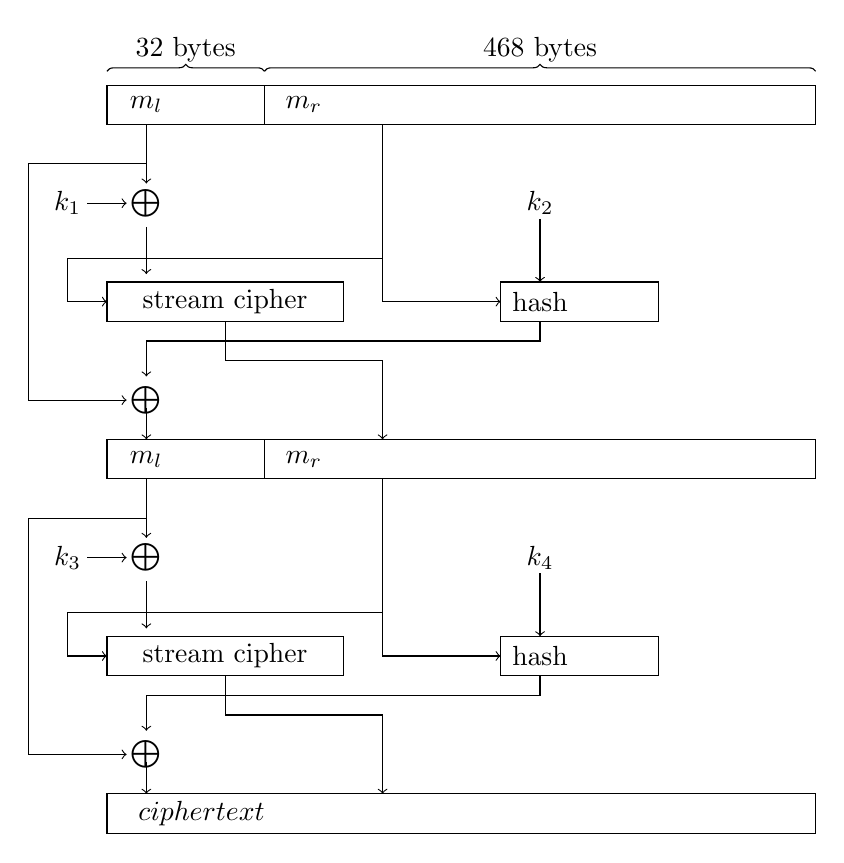
\begin{tikzpicture}
        \def\hashLength{2}
        \def\cipherLength{7}
        \draw[decoration={brace,raise=5pt},decorate] (0,0.5) -- node[above=5pt] {32 bytes} (\hashLength,0.5);
        \draw[decoration={brace,raise=5pt},decorate] (\hashLength,0.5) -- node[above=5pt] {468 bytes} (\hashLength+\cipherLength,0.5);

        \foreach \i\j\offset in{1/2/0,3/4/-4.5} {
                \begin{scope}[shift={(0,\offset)}]
                    \draw (0,0) rectangle (\hashLength,0.5);
                    \draw (\hashLength,0) rectangle (\hashLength+\cipherLength,0.5);

                    \draw (0.5,0.25) node {$m_l$};
                    \draw (\hashLength+0.5,0.25) node {$m_r$};

                    % Encryption
                    \draw (0.5,-1) node {$\bigoplus$};
                    \draw (-0.5,-1) node {$k_\i$};

                    \draw [->] (0.5,0) -- (0.5,-0.75);
                    \draw [->] (-0.25,-1) -- (0.25,-1);
                    \draw [->] (0.5,-1.3) -- (0.5,-1.9);

                    \draw (0,-2.5) rectangle (3, -2);
                    \draw (1.5, -2.25) node [align=center] {stream cipher};

                    % into stream cipher
                    \draw [->] (\hashLength+1.5, 0) -- (\hashLength+1.5, -1.7) -- (-0.5,-1.7) -- (-0.5,-2.25) -- (0,-2.25);

                    \draw [->] (1.5,-2.5) -- (1.5,-3) -- (\hashLength+1.5,-3) -- (\hashLength+1.5,-4);

                    %Hashing
                    \draw (5.5,-1) node {$k_\j$};

                    \draw [->] (5.5,-1.2) -- (5.5,-2);

                    \draw (5,-2.5) rectangle (7, -2);
                    \draw (5.5, -2.25) node [align=center] {hash};

                    \draw [->] (5.5,-2.5) -- (5.5, -2.75) -- (0.5,-2.75) -- (0.5,-3.2);
                    \draw (0.5,-3.5) node {$\bigoplus$};

                    \draw [->] (0.5,-0.5) -- (-1,-0.5) -- (-1,-3.5) -- (0.25,-3.5);
                    \draw [->] (0.5, -3.6) -- (0.5, -4);

                    %m_r into hash
                    \draw [->] (\hashLength+1.5,-1.7) -- (\hashLength+1.5, -2.25) -- (5,-2.25);
                \end{scope}
            }

        \begin{scope}[shift={(0,-9.0)}]
            \draw (0,0) rectangle (\hashLength+\cipherLength,0.5);
            \draw (1.2,0.25) node {$ciphertext$};
        \end{scope}

    \end{tikzpicture}
    \caption{Encryption using LIONESS \cite{lionesspaper} scheme}
\end{figure}